\documentclass[11pt]{article}
\usepackage[textwidth=18.0cm, textheight=23.0cm, top=2.0cm]{geometry}
\usepackage{pst-all}
\usepackage{amssymb}
\usepackage{tikz}
\usepackage{underscore}\begin{document}
\pagestyle{empty}


ClassName: \underline{\textbf{Class_10.2bp-40}}
\par
BinSize: \underline{\textbf{100 × 100}}
\par
ReduceSize: \underline{\textbf{100 × 100}}
\par
TypeNum: \underline{\textbf{98}}
\par
Num: \underline{\textbf{100}}
\par
OutS: \underline{\textbf{140000}}
\par
InS: \underline{\textbf{135996}}
\par
Rate: \underline{\textbf{0.971}}
\par
UB: \underline{\textbf{14}}
\par
LB0: \underline{\textbf{14}}
\par
LB: \underline{\textbf{14}}
\par
LBWithCut: \underline{\textbf{14}}
\par
NodeCut: \underline{\textbf{0}}
\par
ExtendedNodeCnt: \underline{\textbf{1}}
\par
GenNodeCnt: \underline{\textbf{1}}
\par
PrimalNode: \underline{\textbf{0}}
\par
ColumnCount: \underline{\textbf{14}}
\par
TotalCutCount: \underline{\textbf{0}}
\par
RootCutCount: \underline{\textbf{0}}
\par
LPSolverCnt: \underline{\textbf{1}}
\par
PricingSolverCnt: \underline{\textbf{0}}
\par
BranchAndBoundNum: \underline{\textbf{1}}
\par
isOpt: \underline{\textbf{true}}
\par
TimeOnInitSolution: \underline{\textbf{84.850 s}}
\par
TimeOnPrimal: \underline{\textbf{0.000 s}}
\par
TimeOnPricing: \underline{\textbf{0.000 s}}
\par
TimeOnRmp: \underline{\textbf{0.078 s}}
\par
TotalTime: \underline{\textbf{84.990 s}}
\par
\newpage


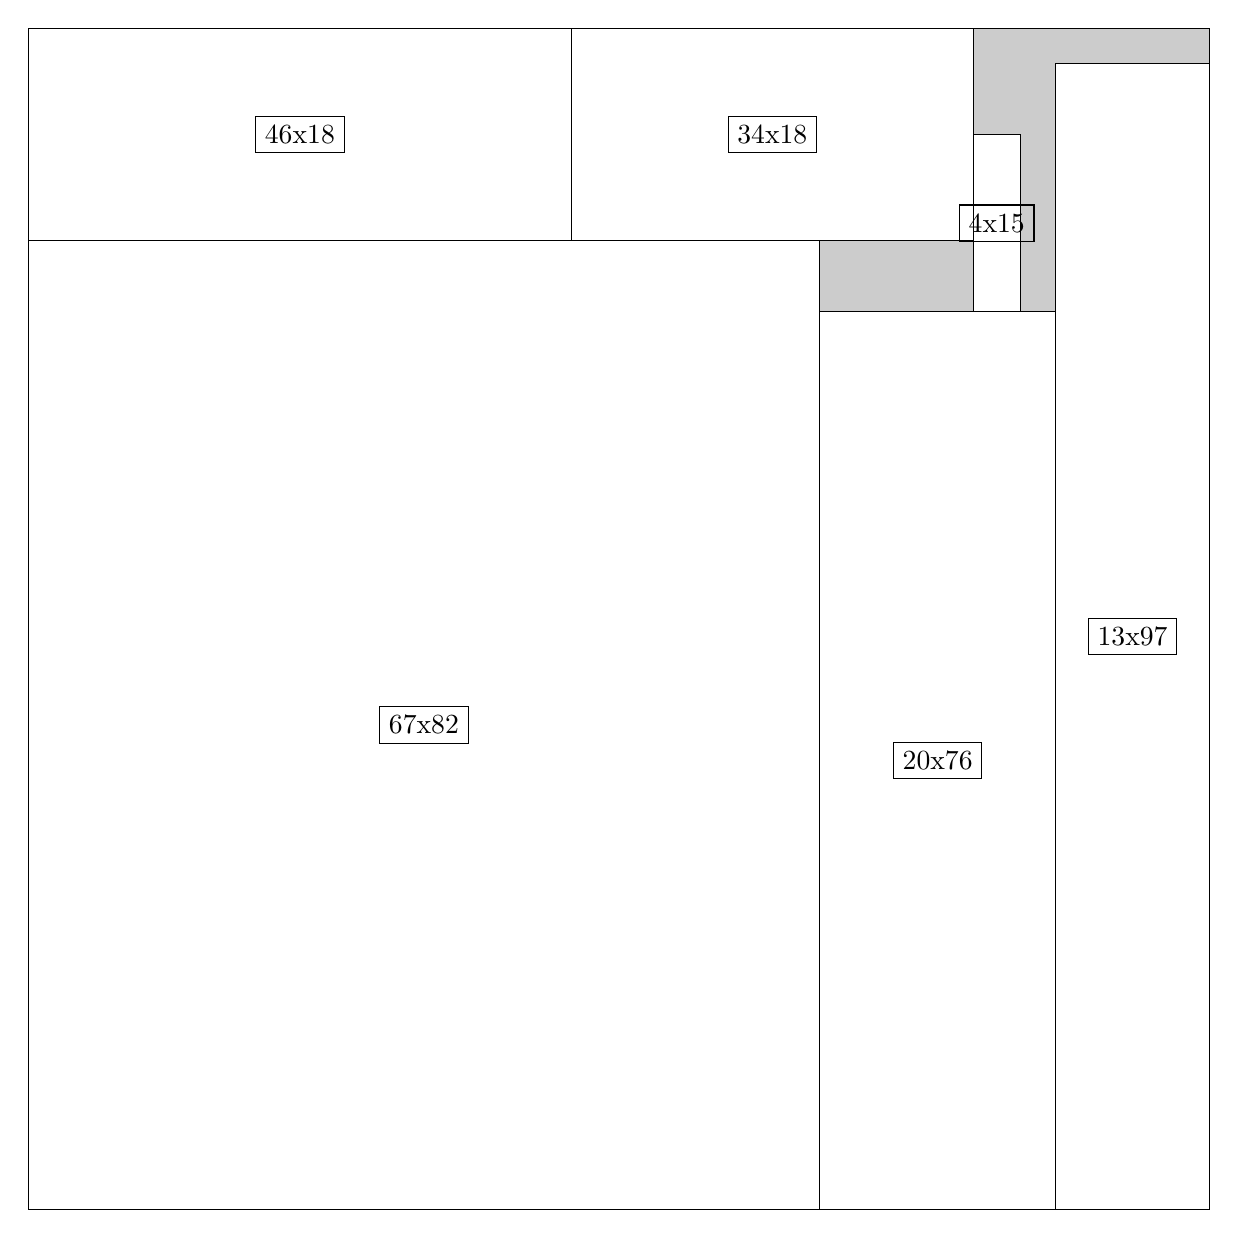
\begin{tikzpicture}[shorten >=1pt,scale=1.0,every node/.style={scale=1.0},->]
\tikzstyle{vertex}=[circle,fill=black!25,minimum size=14pt,inner sep=0pt]
\filldraw[fill=gray!40!white, draw=black] (0,0) rectangle (15.0,15.0);
\foreach \name/\x/\y/\w/\h in {67x82/0.0/0.0/10.049999999999999/12.299999999999999,20x76/10.049999999999999/0.0/3.0/11.4,13x97/13.049999999999999/0.0/1.95/14.549999999999999,46x18/0.0/12.299999999999999/6.8999999999999995/2.6999999999999997,34x18/6.8999999999999995/12.299999999999999/5.1/2.6999999999999997,4x15/12.0/11.4/0.6/2.25}
\filldraw[fill=white!40!white, draw=black] (\x,\y) rectangle node[draw] (\name) {\name} ++(\w,\h);
\end{tikzpicture}


w =67 , h =82 , x =0 , y =0 , v =5494
\par
w =20 , h =76 , x =67 , y =0 , v =1520
\par
w =13 , h =97 , x =87 , y =0 , v =1261
\par
w =46 , h =18 , x =0 , y =82 , v =828
\par
w =34 , h =18 , x =46 , y =82 , v =612
\par
w =4 , h =15 , x =80 , y =76 , v =60
\par
\newpage


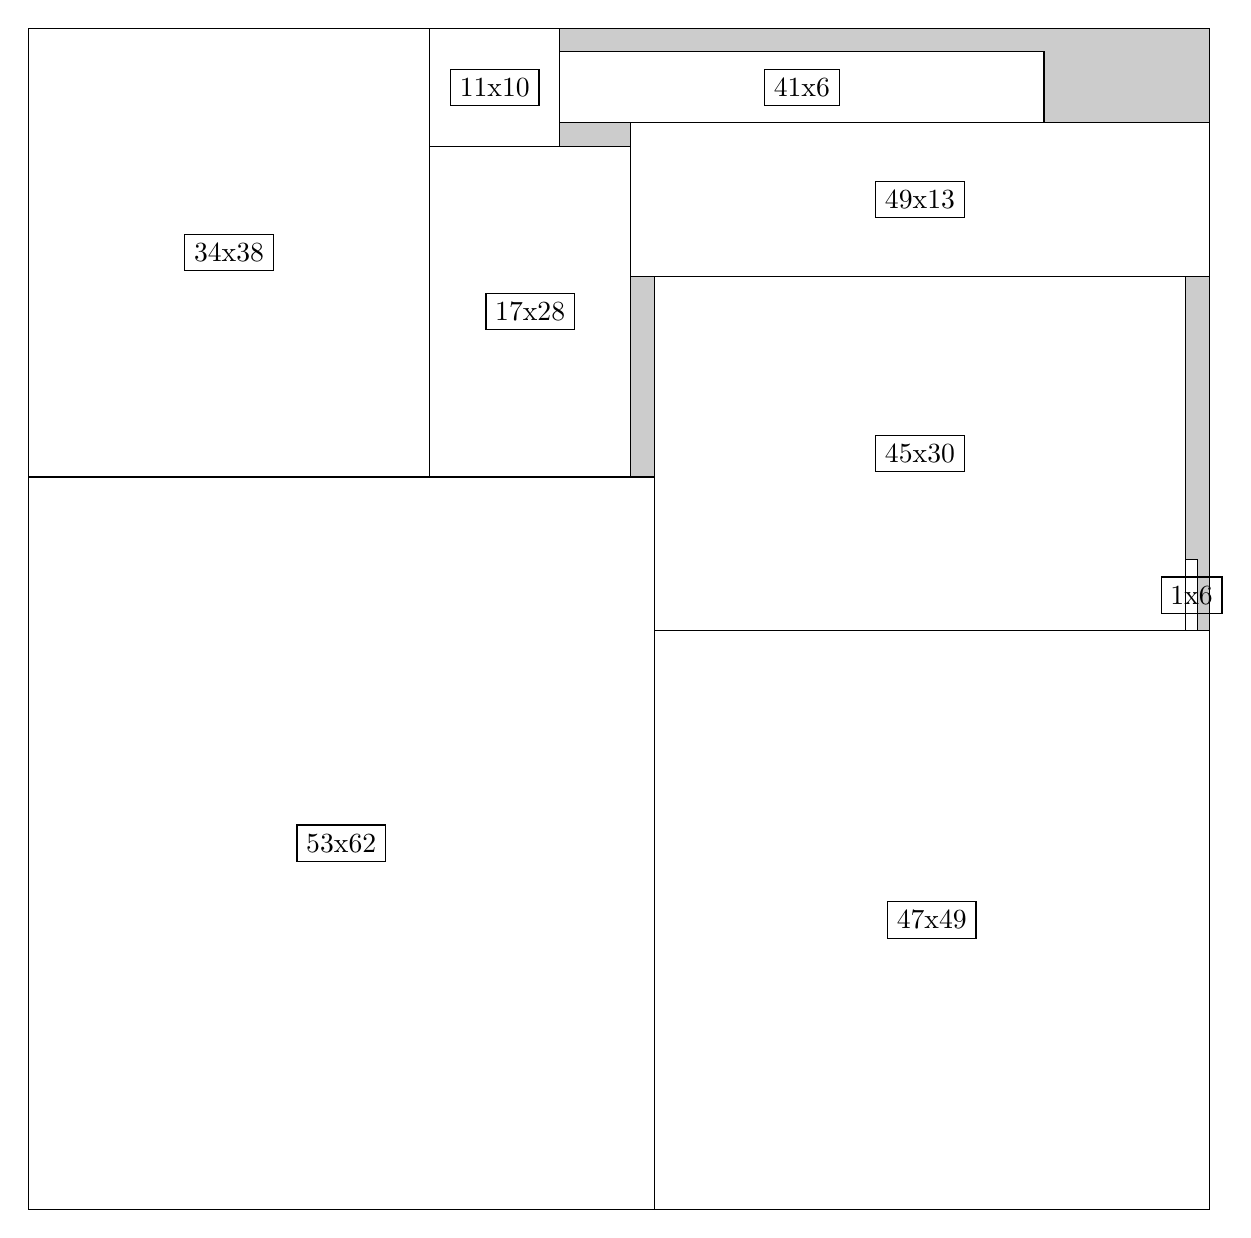
\begin{tikzpicture}[shorten >=1pt,scale=1.0,every node/.style={scale=1.0},->]
\tikzstyle{vertex}=[circle,fill=black!25,minimum size=14pt,inner sep=0pt]
\filldraw[fill=gray!40!white, draw=black] (0,0) rectangle (15.0,15.0);
\foreach \name/\x/\y/\w/\h in {53x62/0.0/0.0/7.949999999999999/9.299999999999999,47x49/7.949999999999999/0.0/7.05/7.35,45x30/7.949999999999999/7.35/6.75/4.5,34x38/0.0/9.299999999999999/5.1/5.7,49x13/7.6499999999999995/11.85/7.35/1.95,17x28/5.1/9.299999999999999/2.55/4.2,41x6/6.75/13.799999999999999/6.1499999999999995/0.8999999999999999,11x10/5.1/13.5/1.65/1.5,1x6/14.7/7.35/0.15/0.8999999999999999}
\filldraw[fill=white!40!white, draw=black] (\x,\y) rectangle node[draw] (\name) {\name} ++(\w,\h);
\end{tikzpicture}


w =53 , h =62 , x =0 , y =0 , v =3286
\par
w =47 , h =49 , x =53 , y =0 , v =2303
\par
w =45 , h =30 , x =53 , y =49 , v =1350
\par
w =34 , h =38 , x =0 , y =62 , v =1292
\par
w =49 , h =13 , x =51 , y =79 , v =637
\par
w =17 , h =28 , x =34 , y =62 , v =476
\par
w =41 , h =6 , x =45 , y =92 , v =246
\par
w =11 , h =10 , x =34 , y =90 , v =110
\par
w =1 , h =6 , x =98 , y =49 , v =6
\par
\newpage


\begin{tikzpicture}[shorten >=1pt,scale=1.0,every node/.style={scale=1.0},->]
\tikzstyle{vertex}=[circle,fill=black!25,minimum size=14pt,inner sep=0pt]
\filldraw[fill=gray!40!white, draw=black] (0,0) rectangle (15.0,15.0);
\foreach \name/\x/\y/\w/\h in {71x96/0.0/0.0/10.65/14.399999999999999,29x41/10.65/0.0/4.35/6.1499999999999995,29x49/10.65/6.1499999999999995/4.35/7.35,29x10/10.65/13.5/4.35/1.5,15x4/7.199999999999999/14.399999999999999/2.25/0.6,48x4/0.0/14.399999999999999/7.199999999999999/0.6}
\filldraw[fill=white!40!white, draw=black] (\x,\y) rectangle node[draw] (\name) {\name} ++(\w,\h);
\end{tikzpicture}


w =71 , h =96 , x =0 , y =0 , v =6816
\par
w =29 , h =41 , x =71 , y =0 , v =1189
\par
w =29 , h =49 , x =71 , y =41 , v =1421
\par
w =29 , h =10 , x =71 , y =90 , v =290
\par
w =15 , h =4 , x =48 , y =96 , v =60
\par
w =48 , h =4 , x =0 , y =96 , v =192
\par
\newpage


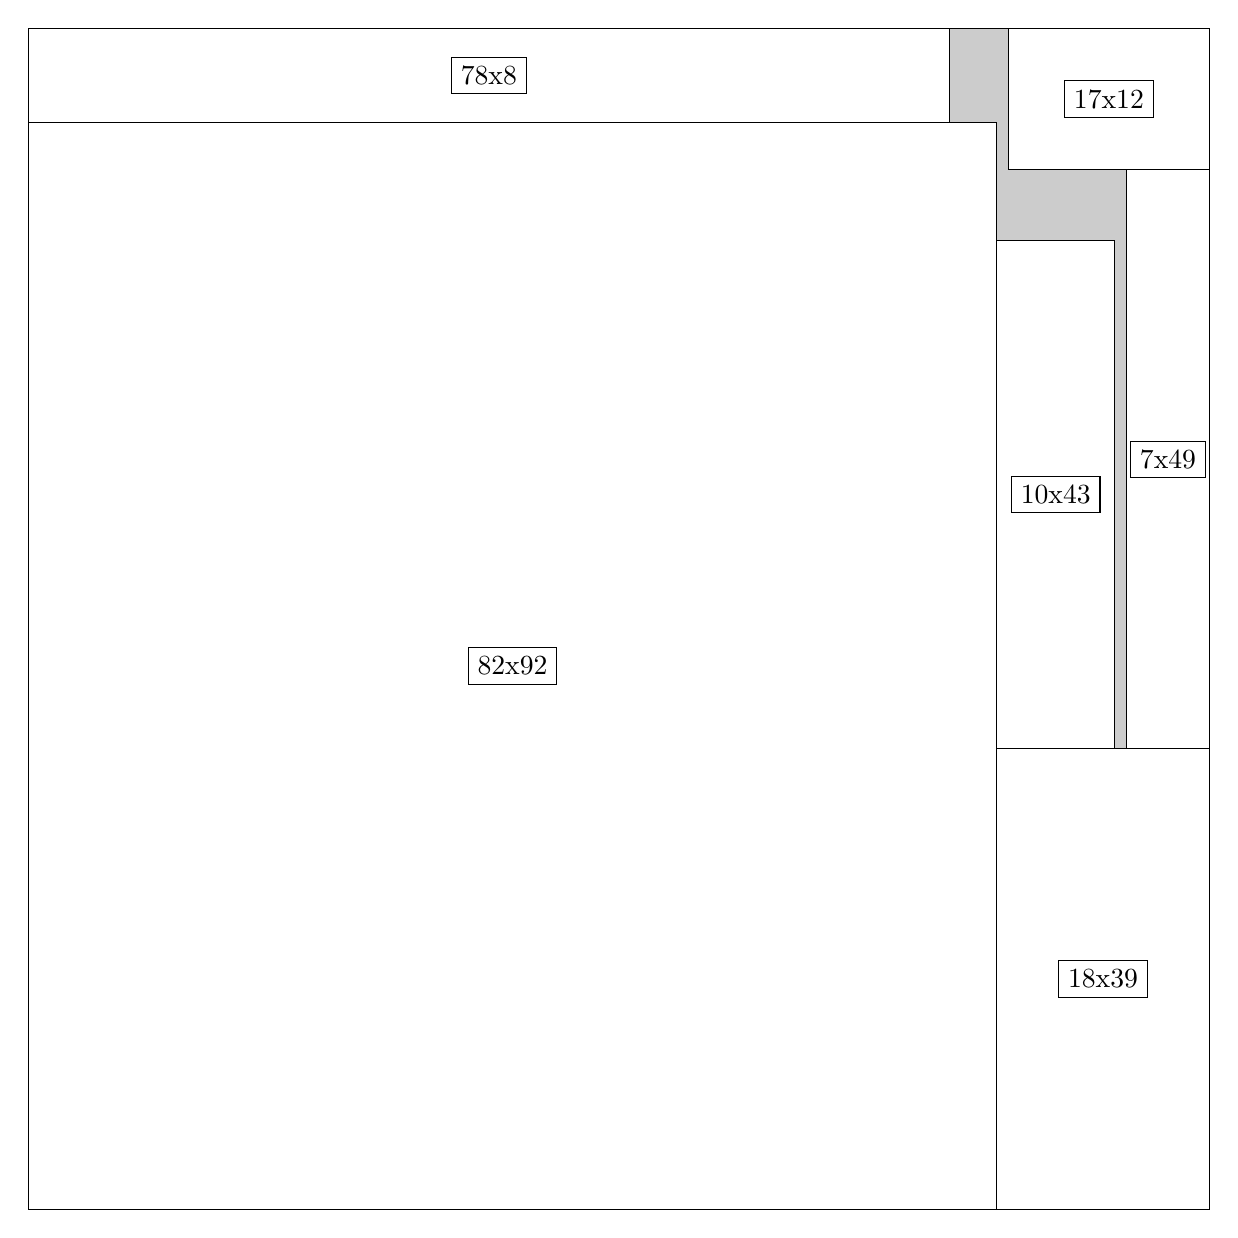
\begin{tikzpicture}[shorten >=1pt,scale=1.0,every node/.style={scale=1.0},->]
\tikzstyle{vertex}=[circle,fill=black!25,minimum size=14pt,inner sep=0pt]
\filldraw[fill=gray!40!white, draw=black] (0,0) rectangle (15.0,15.0);
\foreach \name/\x/\y/\w/\h in {82x92/0.0/0.0/12.299999999999999/13.799999999999999,18x39/12.299999999999999/0.0/2.6999999999999997/5.85,78x8/0.0/13.799999999999999/11.7/1.2,10x43/12.299999999999999/5.85/1.5/6.45,7x49/13.95/5.85/1.05/7.35,17x12/12.45/13.2/2.55/1.7999999999999998}
\filldraw[fill=white!40!white, draw=black] (\x,\y) rectangle node[draw] (\name) {\name} ++(\w,\h);
\end{tikzpicture}


w =82 , h =92 , x =0 , y =0 , v =7544
\par
w =18 , h =39 , x =82 , y =0 , v =702
\par
w =78 , h =8 , x =0 , y =92 , v =624
\par
w =10 , h =43 , x =82 , y =39 , v =430
\par
w =7 , h =49 , x =93 , y =39 , v =343
\par
w =17 , h =12 , x =83 , y =88 , v =204
\par
\newpage


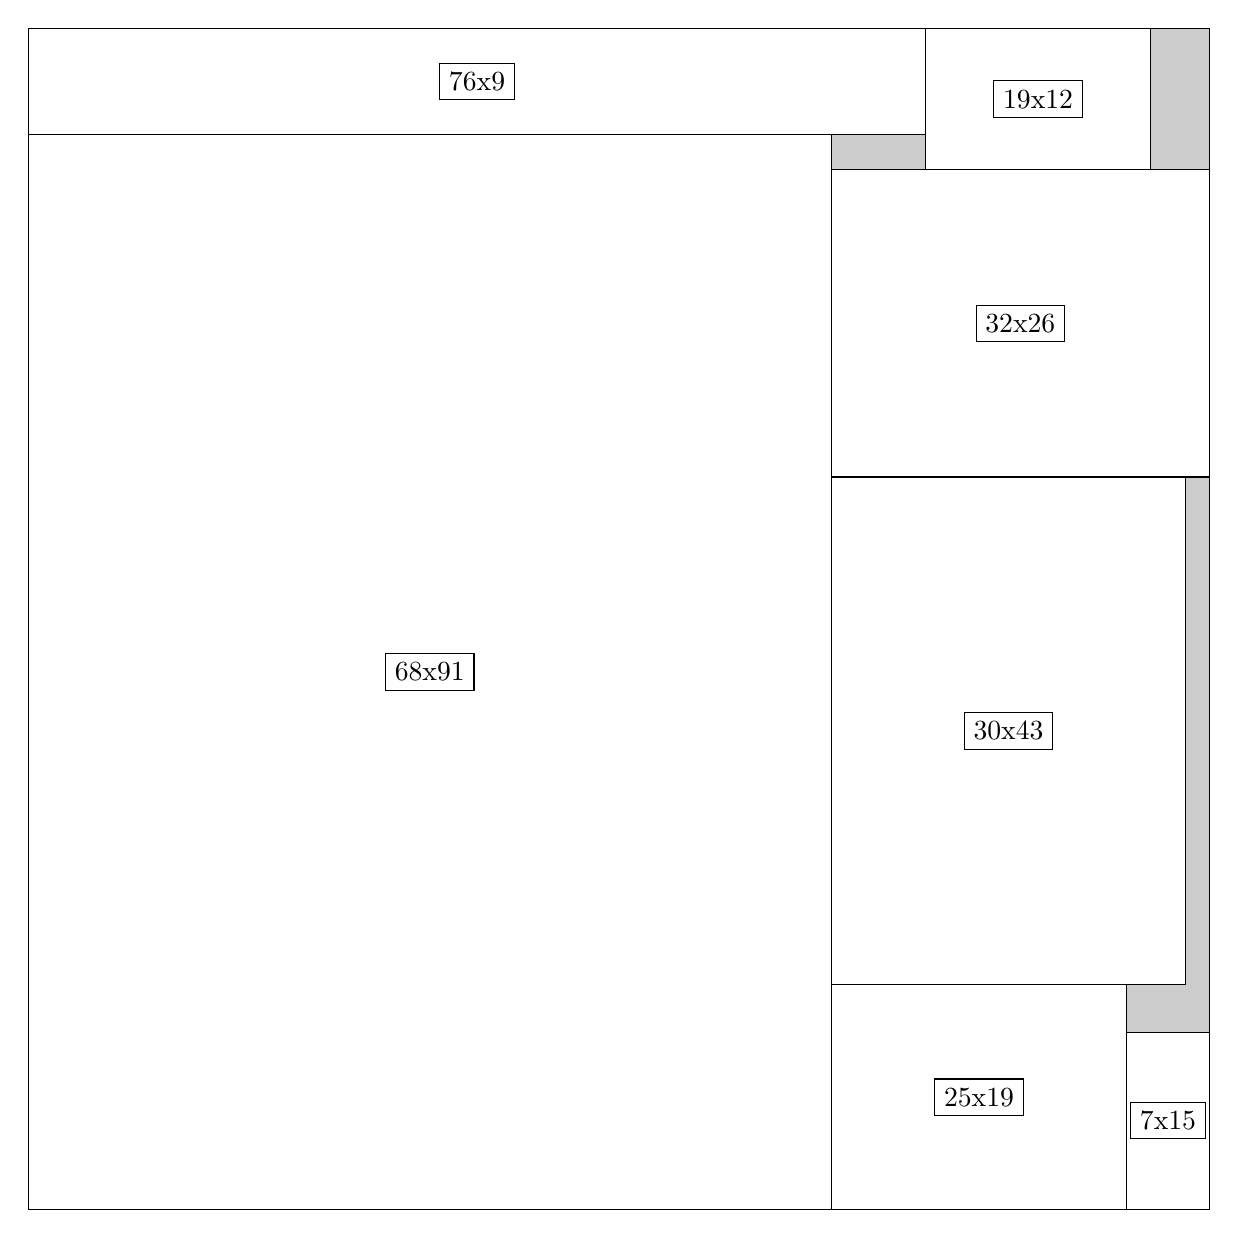
\begin{tikzpicture}[shorten >=1pt,scale=1.0,every node/.style={scale=1.0},->]
\tikzstyle{vertex}=[circle,fill=black!25,minimum size=14pt,inner sep=0pt]
\filldraw[fill=gray!40!white, draw=black] (0,0) rectangle (15.0,15.0);
\foreach \name/\x/\y/\w/\h in {25x19/10.2/0.0/3.75/2.85,30x43/10.2/2.85/4.5/6.45,32x26/10.2/9.299999999999999/4.8/3.9,76x9/0.0/13.65/11.4/1.3499999999999999,7x15/13.95/0.0/1.05/2.25,19x12/11.4/13.2/2.85/1.7999999999999998,68x91/0.0/0.0/10.2/13.65}
\filldraw[fill=white!40!white, draw=black] (\x,\y) rectangle node[draw] (\name) {\name} ++(\w,\h);
\end{tikzpicture}


w =25 , h =19 , x =68 , y =0 , v =475
\par
w =30 , h =43 , x =68 , y =19 , v =1290
\par
w =32 , h =26 , x =68 , y =62 , v =832
\par
w =76 , h =9 , x =0 , y =91 , v =684
\par
w =7 , h =15 , x =93 , y =0 , v =105
\par
w =19 , h =12 , x =76 , y =88 , v =228
\par
w =68 , h =91 , x =0 , y =0 , v =6188
\par
\newpage


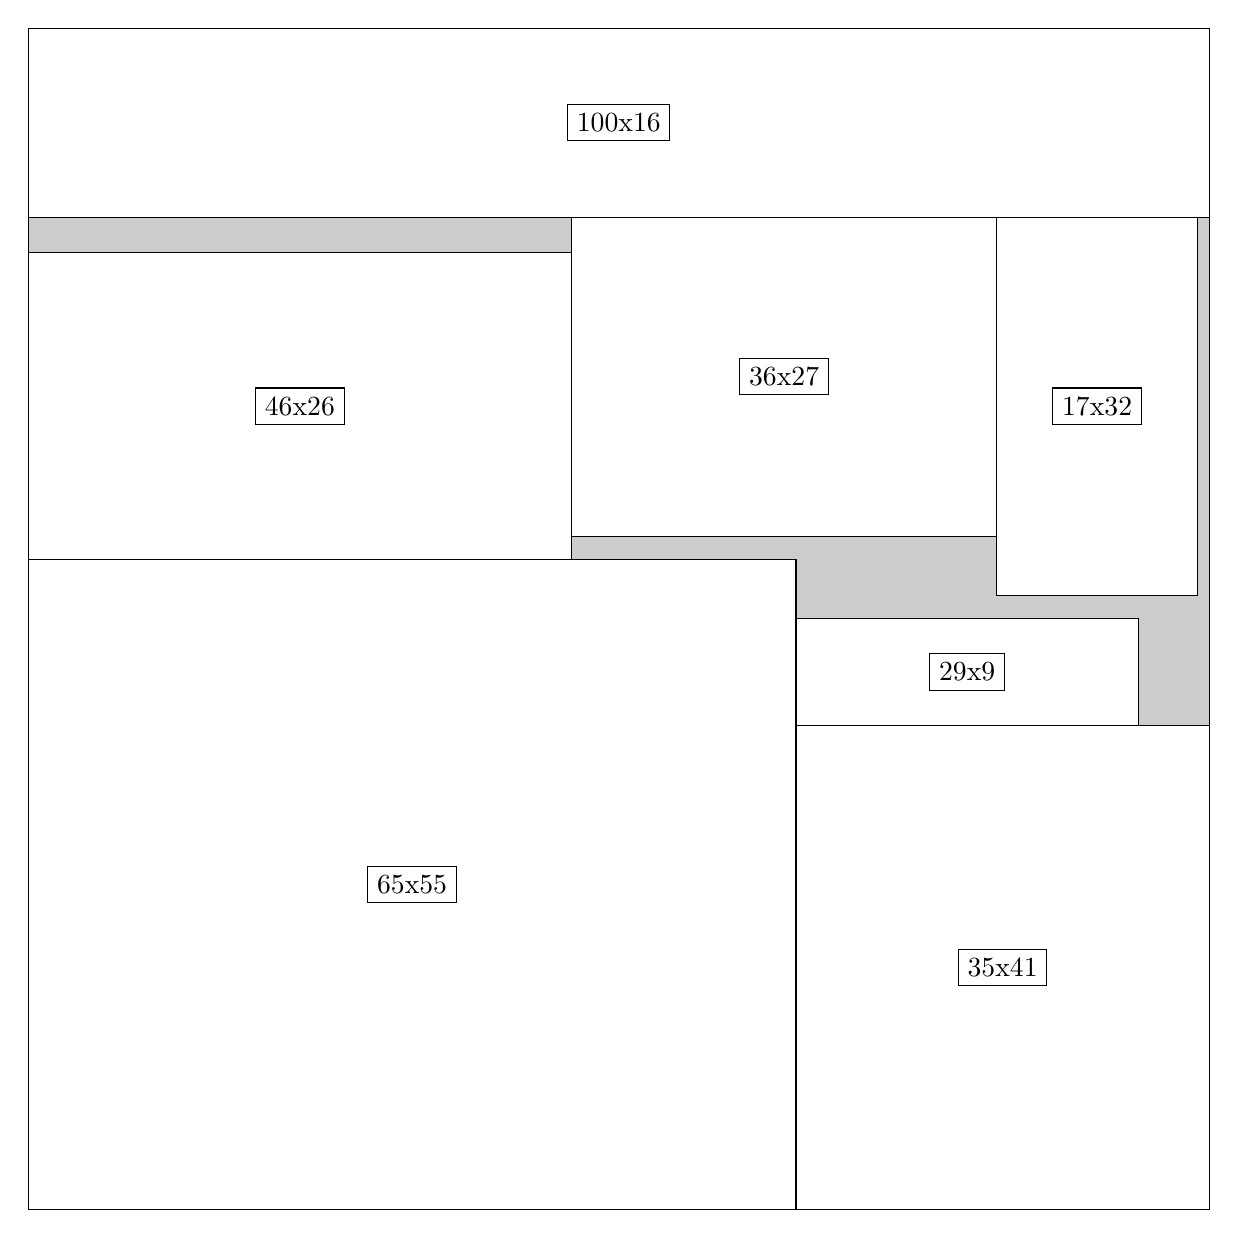
\begin{tikzpicture}[shorten >=1pt,scale=1.0,every node/.style={scale=1.0},->]
\tikzstyle{vertex}=[circle,fill=black!25,minimum size=14pt,inner sep=0pt]
\filldraw[fill=gray!40!white, draw=black] (0,0) rectangle (15.0,15.0);
\foreach \name/\x/\y/\w/\h in {65x55/0.0/0.0/9.75/8.25,100x16/0.0/12.6/15.0/2.4,35x41/9.75/0.0/5.25/6.1499999999999995,46x26/0.0/8.25/6.8999999999999995/3.9,36x27/6.8999999999999995/8.549999999999999/5.3999999999999995/4.05,17x32/12.299999999999999/7.8/2.55/4.8,29x9/9.75/6.1499999999999995/4.35/1.3499999999999999}
\filldraw[fill=white!40!white, draw=black] (\x,\y) rectangle node[draw] (\name) {\name} ++(\w,\h);
\end{tikzpicture}


w =65 , h =55 , x =0 , y =0 , v =3575
\par
w =100 , h =16 , x =0 , y =84 , v =1600
\par
w =35 , h =41 , x =65 , y =0 , v =1435
\par
w =46 , h =26 , x =0 , y =55 , v =1196
\par
w =36 , h =27 , x =46 , y =57 , v =972
\par
w =17 , h =32 , x =82 , y =52 , v =544
\par
w =29 , h =9 , x =65 , y =41 , v =261
\par
\newpage


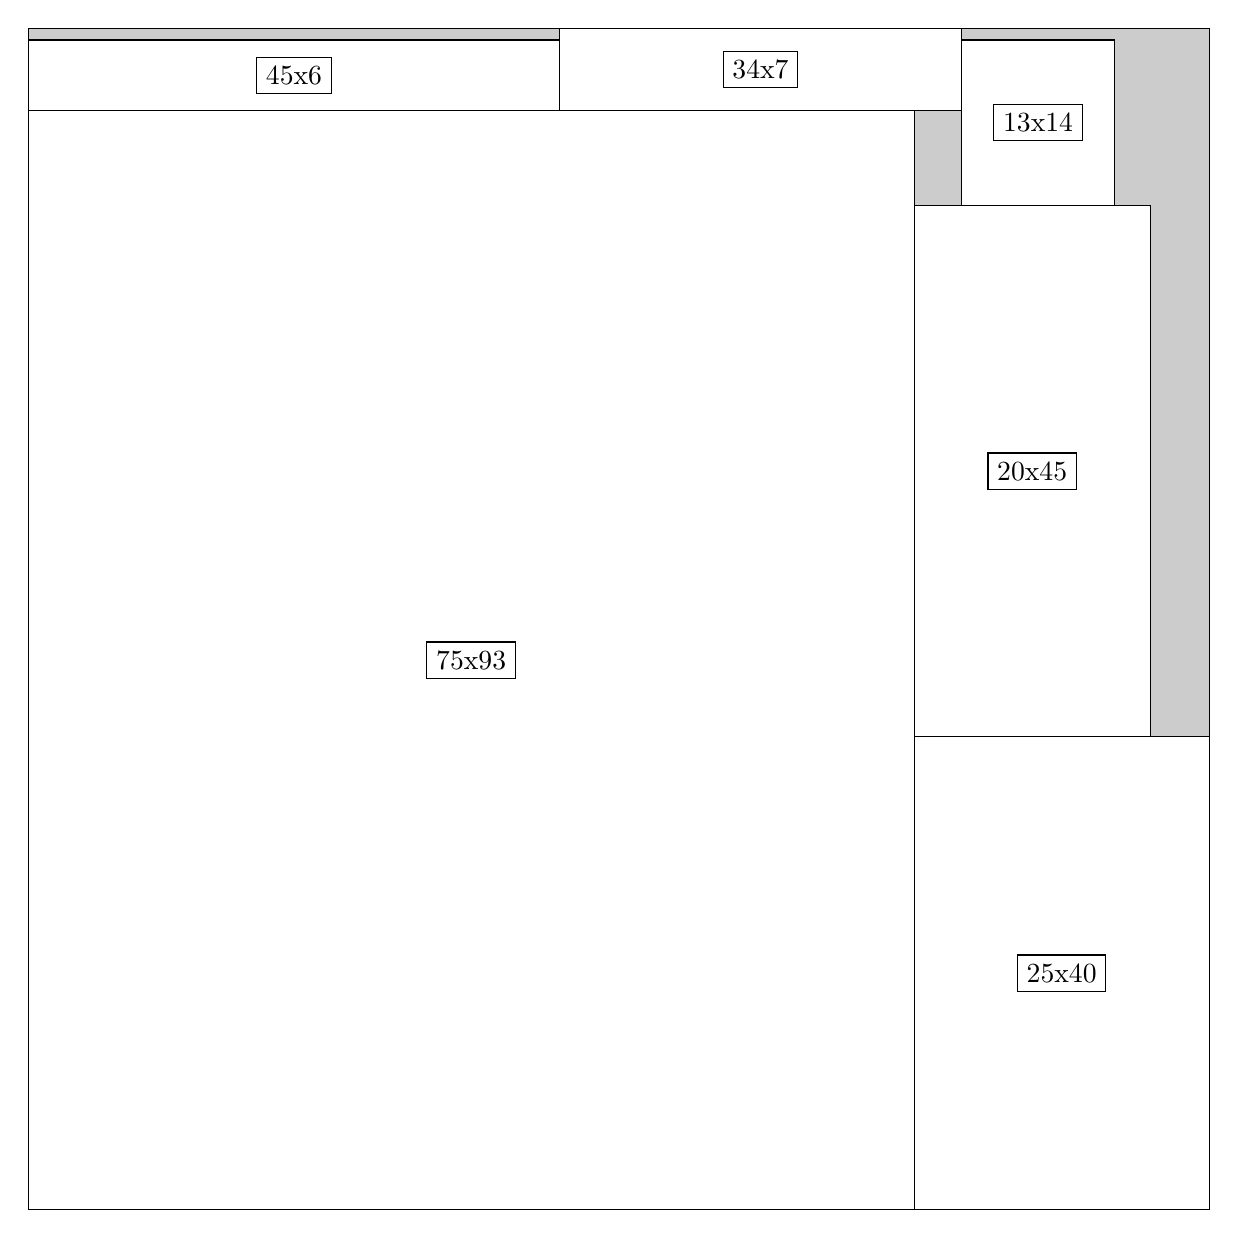
\begin{tikzpicture}[shorten >=1pt,scale=1.0,every node/.style={scale=1.0},->]
\tikzstyle{vertex}=[circle,fill=black!25,minimum size=14pt,inner sep=0pt]
\filldraw[fill=gray!40!white, draw=black] (0,0) rectangle (15.0,15.0);
\foreach \name/\x/\y/\w/\h in {75x93/0.0/0.0/11.25/13.95,25x40/11.25/0.0/3.75/6.0,20x45/11.25/6.0/3.0/6.75,45x6/0.0/13.95/6.75/0.8999999999999999,34x7/6.75/13.95/5.1/1.05,13x14/11.85/12.75/1.95/2.1}
\filldraw[fill=white!40!white, draw=black] (\x,\y) rectangle node[draw] (\name) {\name} ++(\w,\h);
\end{tikzpicture}


w =75 , h =93 , x =0 , y =0 , v =6975
\par
w =25 , h =40 , x =75 , y =0 , v =1000
\par
w =20 , h =45 , x =75 , y =40 , v =900
\par
w =45 , h =6 , x =0 , y =93 , v =270
\par
w =34 , h =7 , x =45 , y =93 , v =238
\par
w =13 , h =14 , x =79 , y =85 , v =182
\par
\newpage


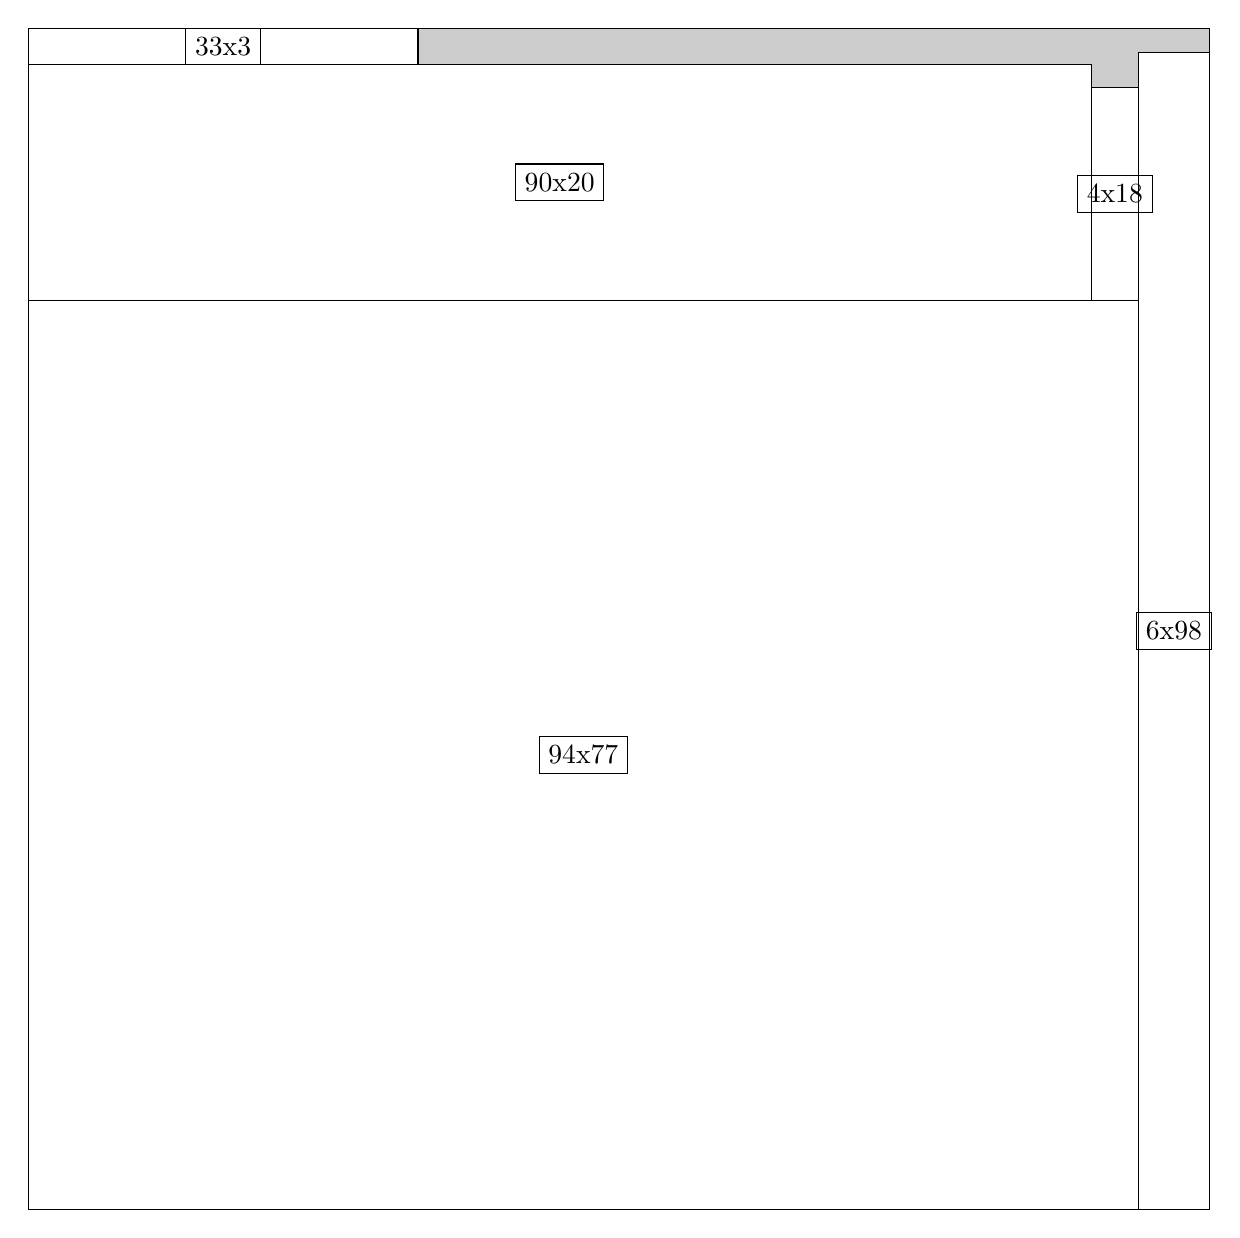
\begin{tikzpicture}[shorten >=1pt,scale=1.0,every node/.style={scale=1.0},->]
\tikzstyle{vertex}=[circle,fill=black!25,minimum size=14pt,inner sep=0pt]
\filldraw[fill=gray!40!white, draw=black] (0,0) rectangle (15.0,15.0);
\foreach \name/\x/\y/\w/\h in {94x77/0.0/0.0/14.1/11.549999999999999,90x20/0.0/11.549999999999999/13.5/3.0,6x98/14.1/0.0/0.8999999999999999/14.7,33x3/0.0/14.549999999999999/4.95/0.44999999999999996,4x18/13.5/11.549999999999999/0.6/2.6999999999999997}
\filldraw[fill=white!40!white, draw=black] (\x,\y) rectangle node[draw] (\name) {\name} ++(\w,\h);
\end{tikzpicture}


w =94 , h =77 , x =0 , y =0 , v =7238
\par
w =90 , h =20 , x =0 , y =77 , v =1800
\par
w =6 , h =98 , x =94 , y =0 , v =588
\par
w =33 , h =3 , x =0 , y =97 , v =99
\par
w =4 , h =18 , x =90 , y =77 , v =72
\par
\newpage


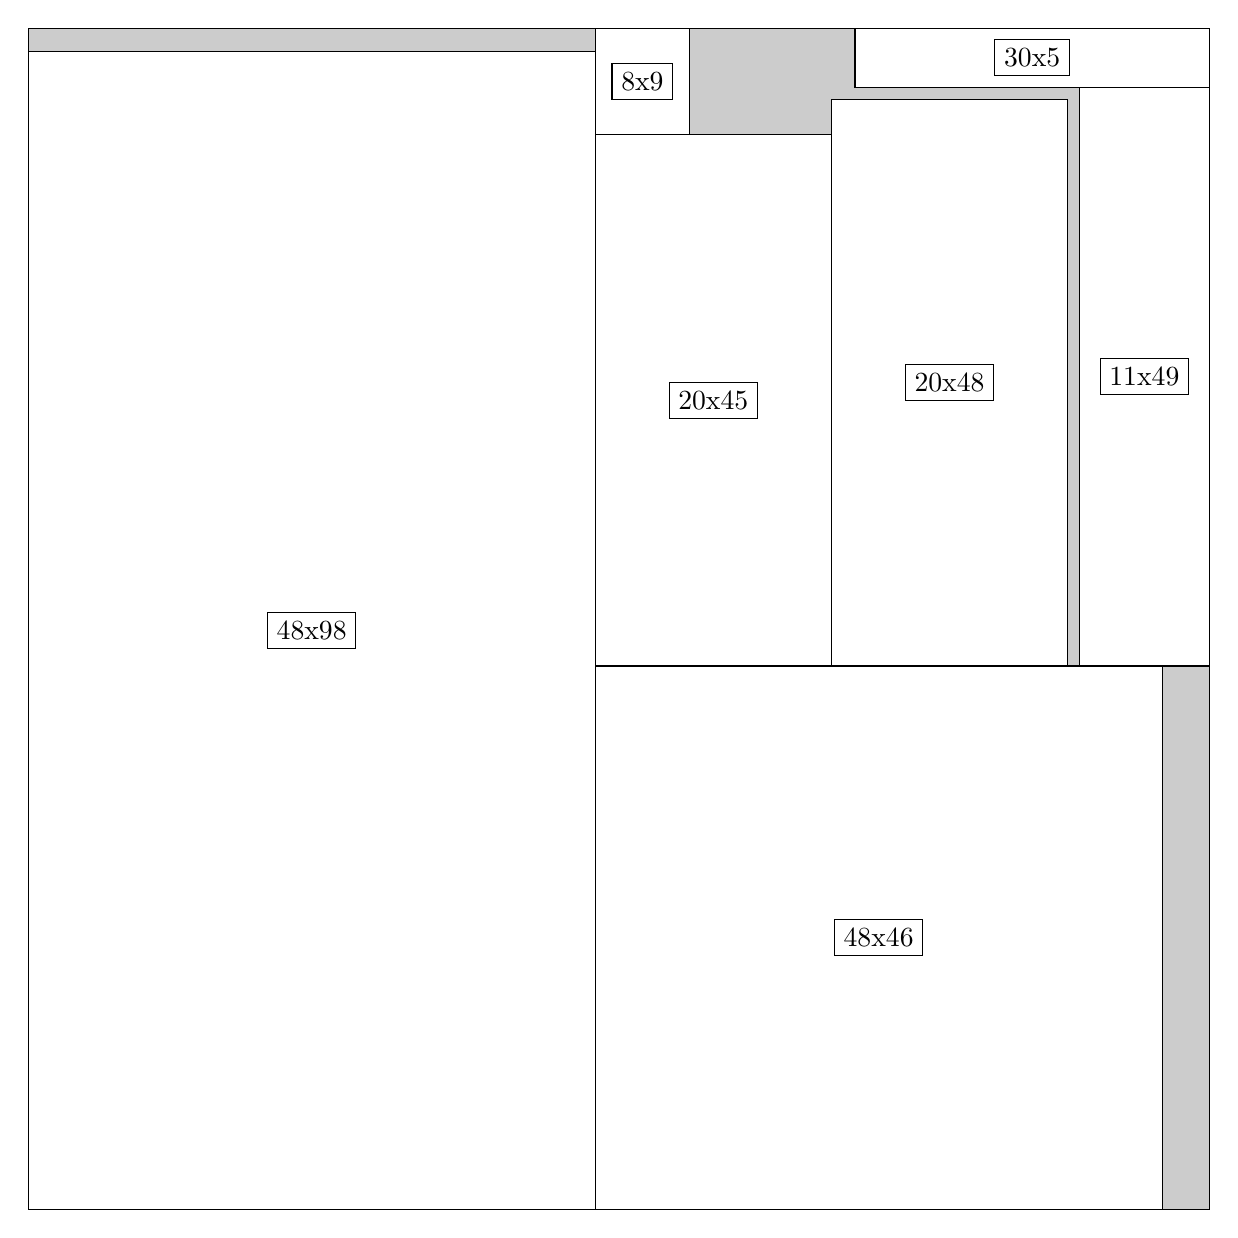
\begin{tikzpicture}[shorten >=1pt,scale=1.0,every node/.style={scale=1.0},->]
\tikzstyle{vertex}=[circle,fill=black!25,minimum size=14pt,inner sep=0pt]
\filldraw[fill=gray!40!white, draw=black] (0,0) rectangle (15.0,15.0);
\foreach \name/\x/\y/\w/\h in {48x98/0.0/0.0/7.199999999999999/14.7,48x46/7.199999999999999/0.0/7.199999999999999/6.8999999999999995,20x48/10.2/6.8999999999999995/3.0/7.199999999999999,11x49/13.35/6.8999999999999995/1.65/7.35,20x45/7.199999999999999/6.8999999999999995/3.0/6.75,30x5/10.5/14.25/4.5/0.75,8x9/7.199999999999999/13.65/1.2/1.3499999999999999}
\filldraw[fill=white!40!white, draw=black] (\x,\y) rectangle node[draw] (\name) {\name} ++(\w,\h);
\end{tikzpicture}


w =48 , h =98 , x =0 , y =0 , v =4704
\par
w =48 , h =46 , x =48 , y =0 , v =2208
\par
w =20 , h =48 , x =68 , y =46 , v =960
\par
w =11 , h =49 , x =89 , y =46 , v =539
\par
w =20 , h =45 , x =48 , y =46 , v =900
\par
w =30 , h =5 , x =70 , y =95 , v =150
\par
w =8 , h =9 , x =48 , y =91 , v =72
\par
\newpage


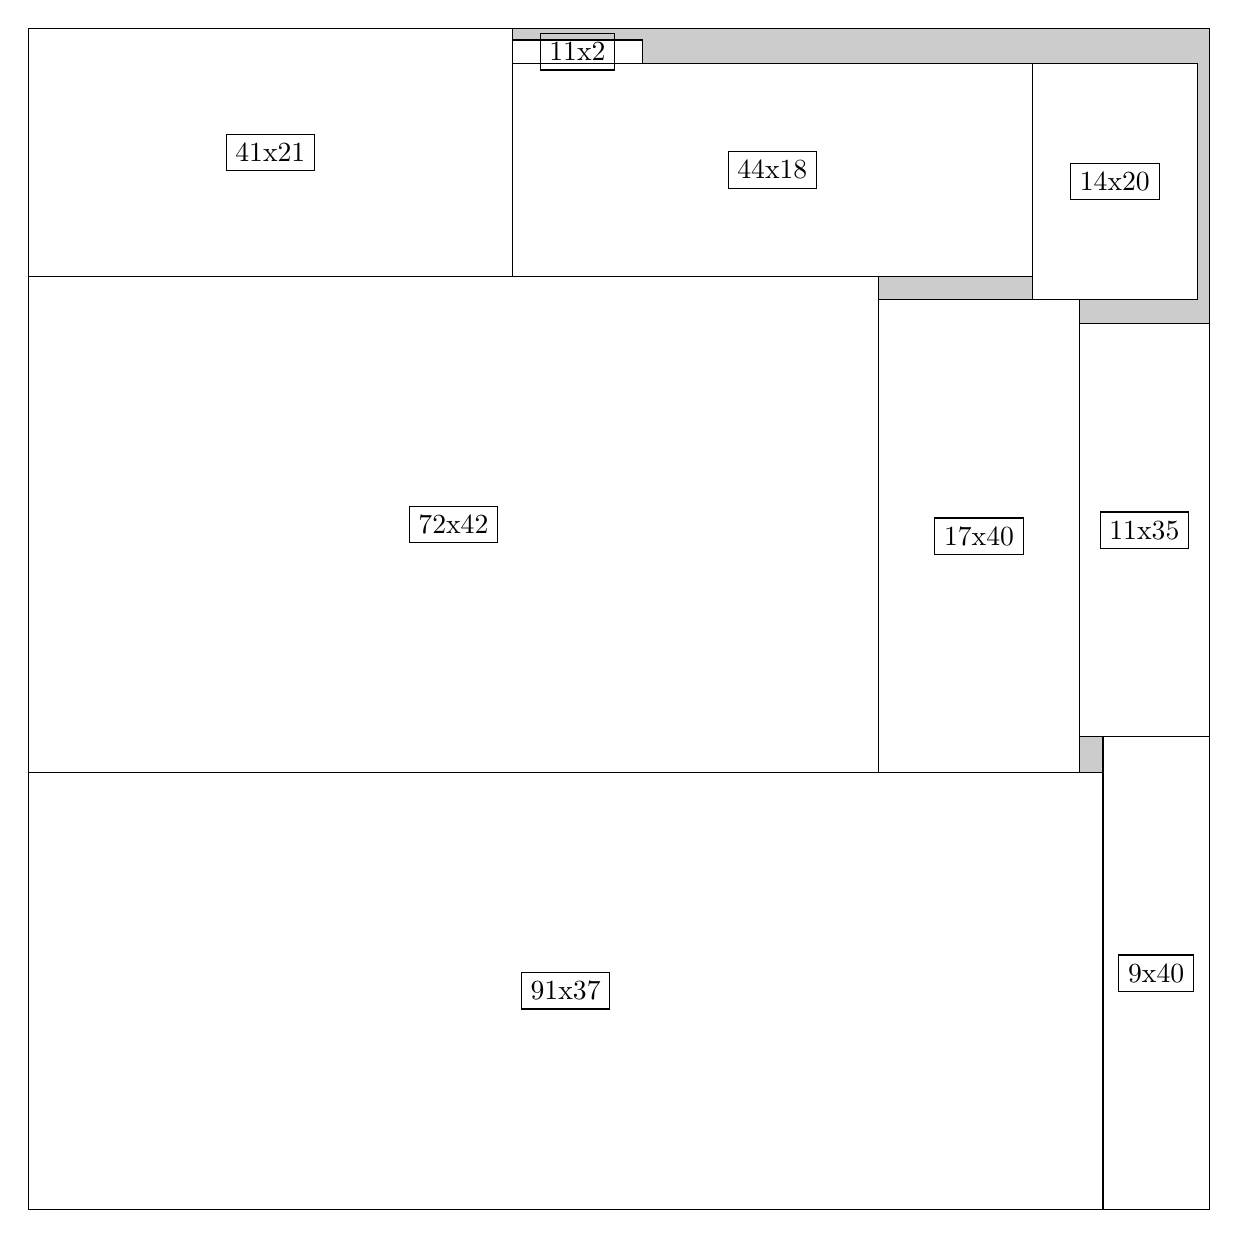
\begin{tikzpicture}[shorten >=1pt,scale=1.0,every node/.style={scale=1.0},->]
\tikzstyle{vertex}=[circle,fill=black!25,minimum size=14pt,inner sep=0pt]
\filldraw[fill=gray!40!white, draw=black] (0,0) rectangle (15.0,15.0);
\foreach \name/\x/\y/\w/\h in {91x37/0.0/0.0/13.65/5.55,72x42/0.0/5.55/10.799999999999999/6.3,41x21/0.0/11.85/6.1499999999999995/3.15,17x40/10.799999999999999/5.55/2.55/6.0,44x18/6.1499999999999995/11.85/6.6/2.6999999999999997,9x40/13.65/0.0/1.3499999999999999/6.0,11x35/13.35/6.0/1.65/5.25,14x20/12.75/11.549999999999999/2.1/3.0,11x2/6.1499999999999995/14.549999999999999/1.65/0.3}
\filldraw[fill=white!40!white, draw=black] (\x,\y) rectangle node[draw] (\name) {\name} ++(\w,\h);
\end{tikzpicture}


w =91 , h =37 , x =0 , y =0 , v =3367
\par
w =72 , h =42 , x =0 , y =37 , v =3024
\par
w =41 , h =21 , x =0 , y =79 , v =861
\par
w =17 , h =40 , x =72 , y =37 , v =680
\par
w =44 , h =18 , x =41 , y =79 , v =792
\par
w =9 , h =40 , x =91 , y =0 , v =360
\par
w =11 , h =35 , x =89 , y =40 , v =385
\par
w =14 , h =20 , x =85 , y =77 , v =280
\par
w =11 , h =2 , x =41 , y =97 , v =22
\par
\newpage


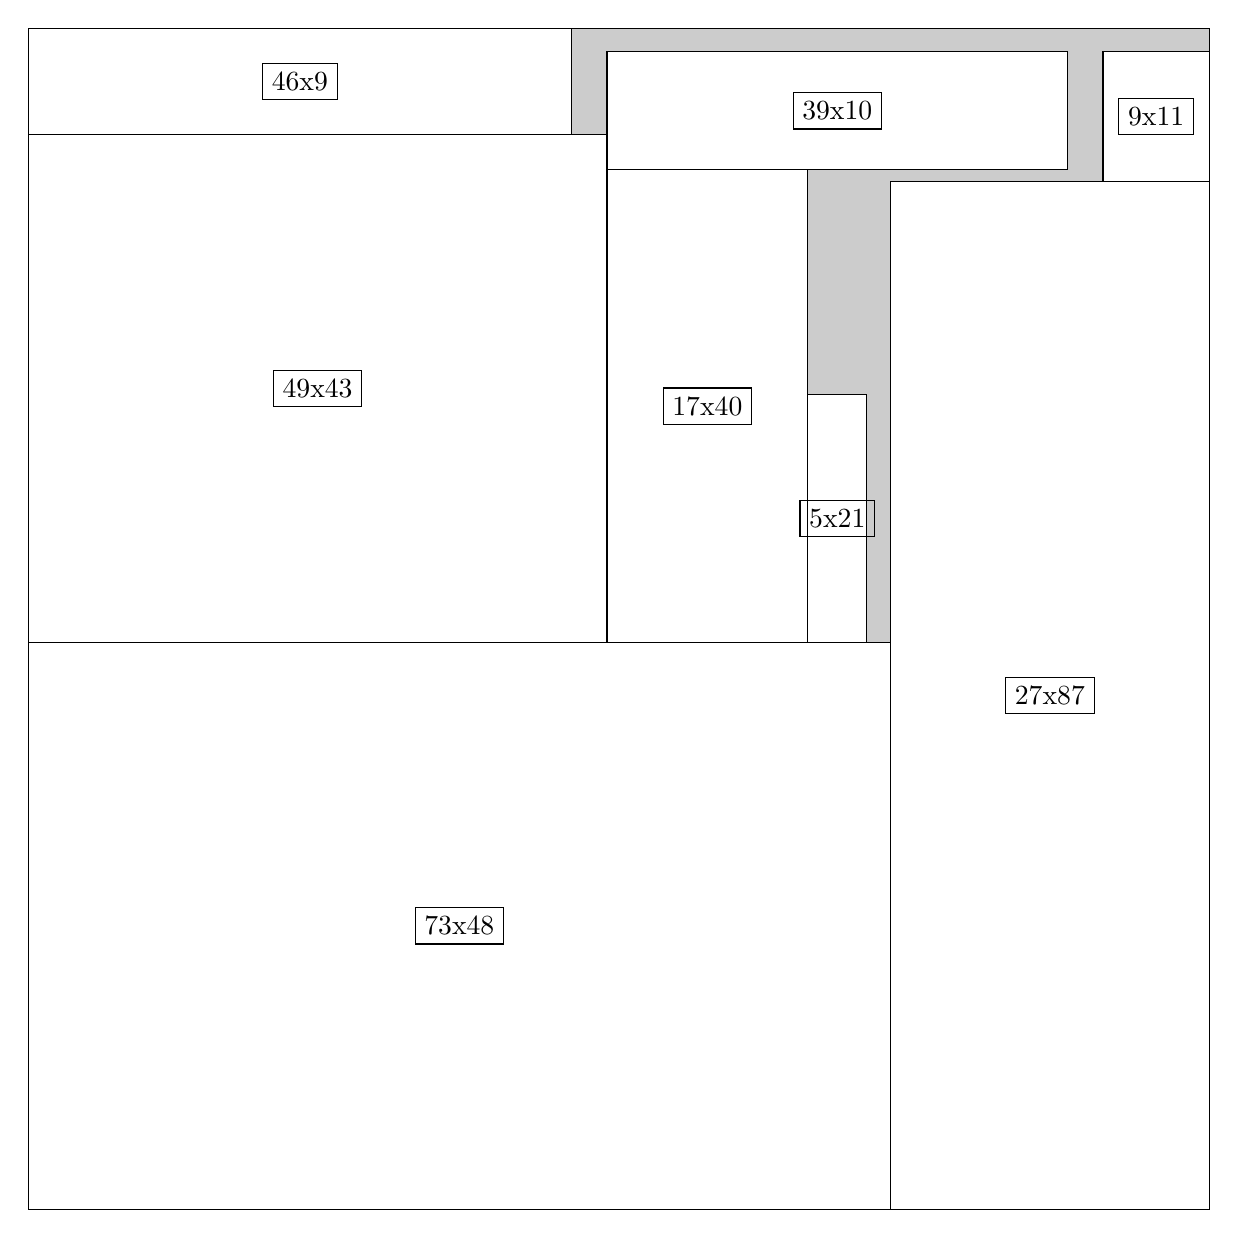
\begin{tikzpicture}[shorten >=1pt,scale=1.0,every node/.style={scale=1.0},->]
\tikzstyle{vertex}=[circle,fill=black!25,minimum size=14pt,inner sep=0pt]
\filldraw[fill=gray!40!white, draw=black] (0,0) rectangle (15.0,15.0);
\foreach \name/\x/\y/\w/\h in {73x48/0.0/0.0/10.95/7.199999999999999,27x87/10.95/0.0/4.05/13.049999999999999,49x43/0.0/7.199999999999999/7.35/6.45,17x40/7.35/7.199999999999999/2.55/6.0,46x9/0.0/13.65/6.8999999999999995/1.3499999999999999,39x10/7.35/13.2/5.85/1.5,5x21/9.9/7.199999999999999/0.75/3.15,9x11/13.65/13.049999999999999/1.3499999999999999/1.65}
\filldraw[fill=white!40!white, draw=black] (\x,\y) rectangle node[draw] (\name) {\name} ++(\w,\h);
\end{tikzpicture}


w =73 , h =48 , x =0 , y =0 , v =3504
\par
w =27 , h =87 , x =73 , y =0 , v =2349
\par
w =49 , h =43 , x =0 , y =48 , v =2107
\par
w =17 , h =40 , x =49 , y =48 , v =680
\par
w =46 , h =9 , x =0 , y =91 , v =414
\par
w =39 , h =10 , x =49 , y =88 , v =390
\par
w =5 , h =21 , x =66 , y =48 , v =105
\par
w =9 , h =11 , x =91 , y =87 , v =99
\par
\newpage


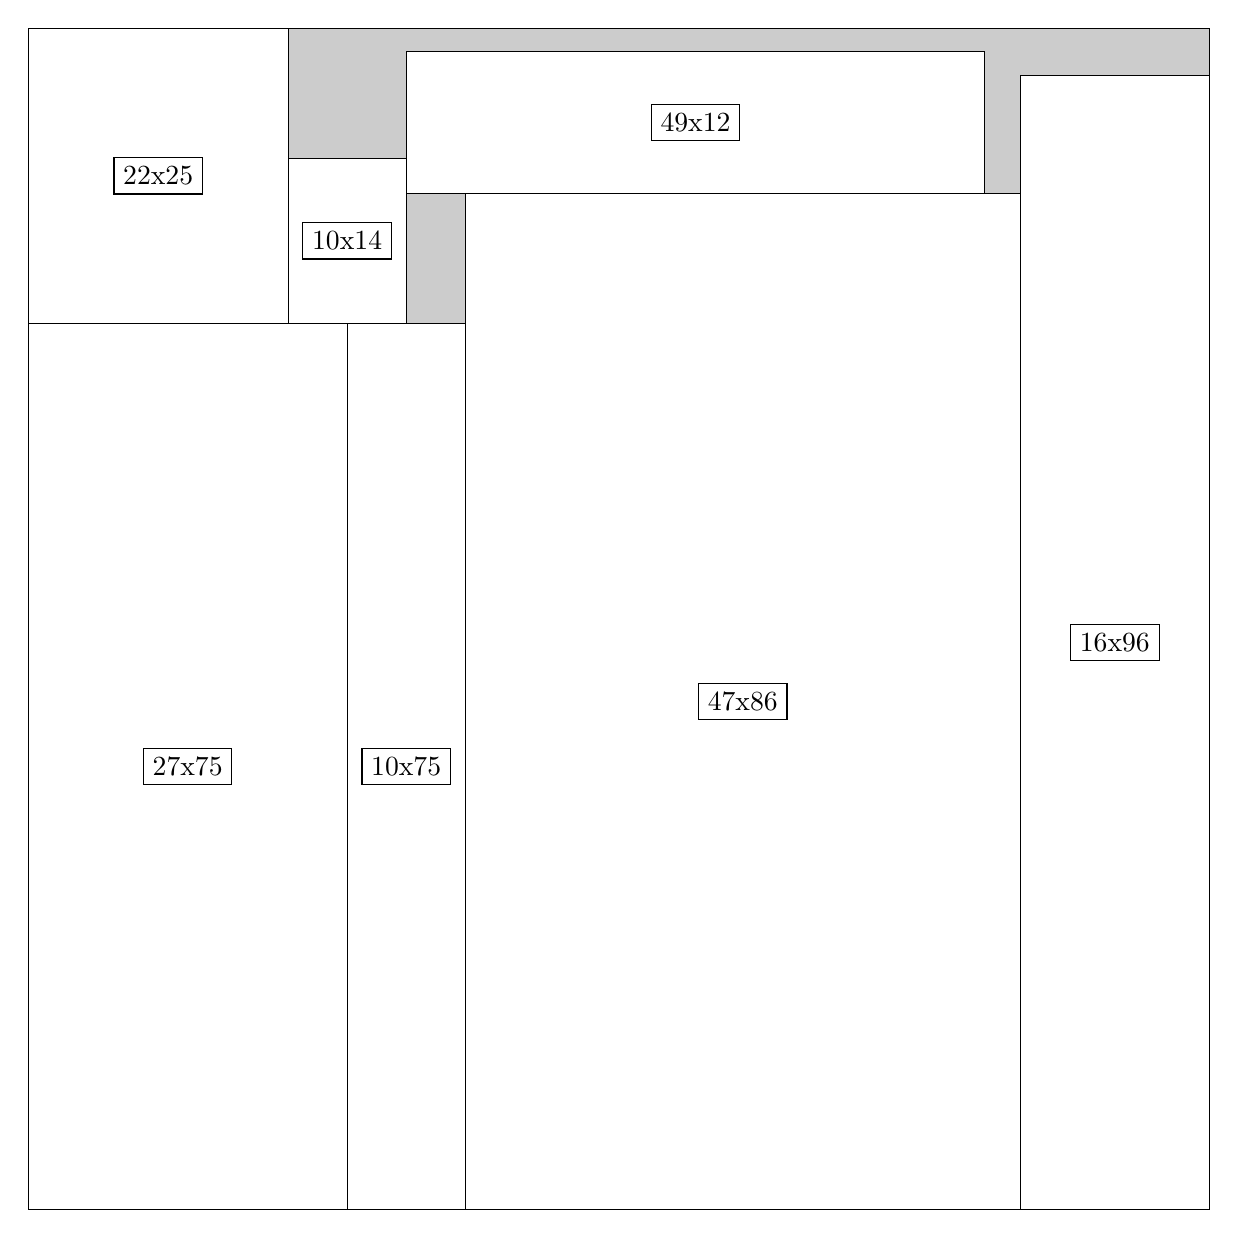
\begin{tikzpicture}[shorten >=1pt,scale=1.0,every node/.style={scale=1.0},->]
\tikzstyle{vertex}=[circle,fill=black!25,minimum size=14pt,inner sep=0pt]
\filldraw[fill=gray!40!white, draw=black] (0,0) rectangle (15.0,15.0);
\foreach \name/\x/\y/\w/\h in {27x75/0.0/0.0/4.05/11.25,47x86/5.55/0.0/7.05/12.9,10x75/4.05/0.0/1.5/11.25,49x12/4.8/12.9/7.35/1.7999999999999998,22x25/0.0/11.25/3.3/3.75,16x96/12.6/0.0/2.4/14.399999999999999,10x14/3.3/11.25/1.5/2.1}
\filldraw[fill=white!40!white, draw=black] (\x,\y) rectangle node[draw] (\name) {\name} ++(\w,\h);
\end{tikzpicture}


w =27 , h =75 , x =0 , y =0 , v =2025
\par
w =47 , h =86 , x =37 , y =0 , v =4042
\par
w =10 , h =75 , x =27 , y =0 , v =750
\par
w =49 , h =12 , x =32 , y =86 , v =588
\par
w =22 , h =25 , x =0 , y =75 , v =550
\par
w =16 , h =96 , x =84 , y =0 , v =1536
\par
w =10 , h =14 , x =22 , y =75 , v =140
\par
\newpage


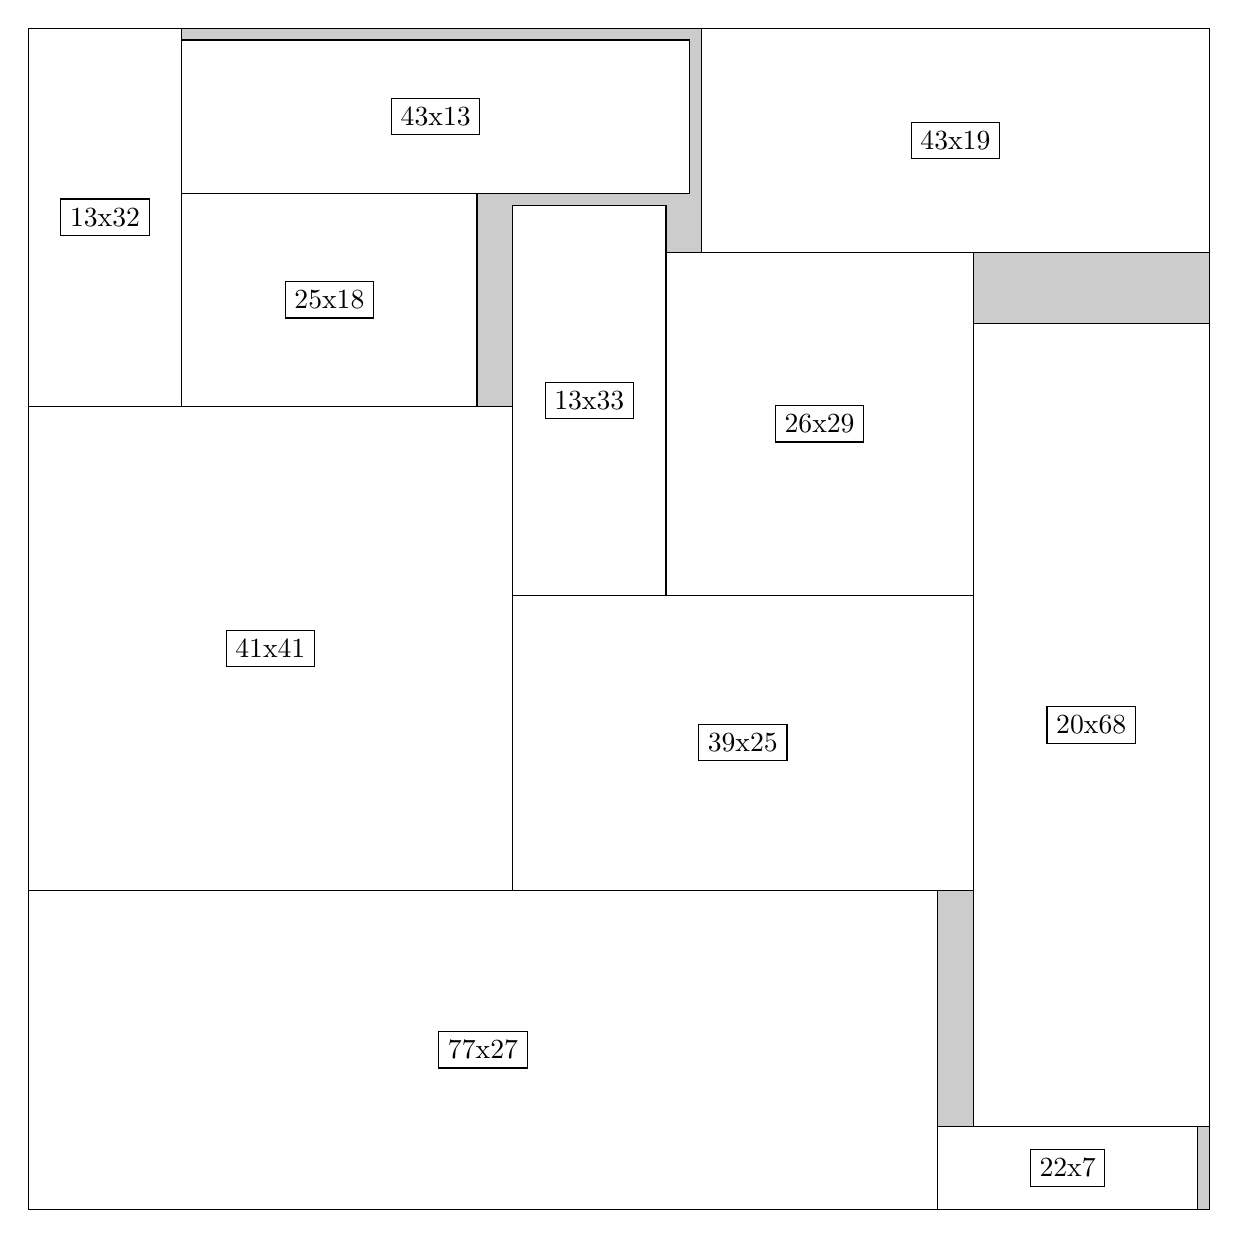
\begin{tikzpicture}[shorten >=1pt,scale=1.0,every node/.style={scale=1.0},->]
\tikzstyle{vertex}=[circle,fill=black!25,minimum size=14pt,inner sep=0pt]
\filldraw[fill=gray!40!white, draw=black] (0,0) rectangle (15.0,15.0);
\foreach \name/\x/\y/\w/\h in {77x27/0.0/0.0/11.549999999999999/4.05,41x41/0.0/4.05/6.1499999999999995/6.1499999999999995,13x33/6.1499999999999995/7.8/1.95/4.95,20x68/12.0/1.05/3.0/10.2,39x25/6.1499999999999995/4.05/5.85/3.75,43x19/8.549999999999999/12.15/6.45/2.85,26x29/8.1/7.8/3.9/4.35,43x13/1.95/12.9/6.45/1.95,25x18/1.95/10.2/3.75/2.6999999999999997,13x32/0.0/10.2/1.95/4.8,22x7/11.549999999999999/0.0/3.3/1.05}
\filldraw[fill=white!40!white, draw=black] (\x,\y) rectangle node[draw] (\name) {\name} ++(\w,\h);
\end{tikzpicture}


w =77 , h =27 , x =0 , y =0 , v =2079
\par
w =41 , h =41 , x =0 , y =27 , v =1681
\par
w =13 , h =33 , x =41 , y =52 , v =429
\par
w =20 , h =68 , x =80 , y =7 , v =1360
\par
w =39 , h =25 , x =41 , y =27 , v =975
\par
w =43 , h =19 , x =57 , y =81 , v =817
\par
w =26 , h =29 , x =54 , y =52 , v =754
\par
w =43 , h =13 , x =13 , y =86 , v =559
\par
w =25 , h =18 , x =13 , y =68 , v =450
\par
w =13 , h =32 , x =0 , y =68 , v =416
\par
w =22 , h =7 , x =77 , y =0 , v =154
\par
\newpage


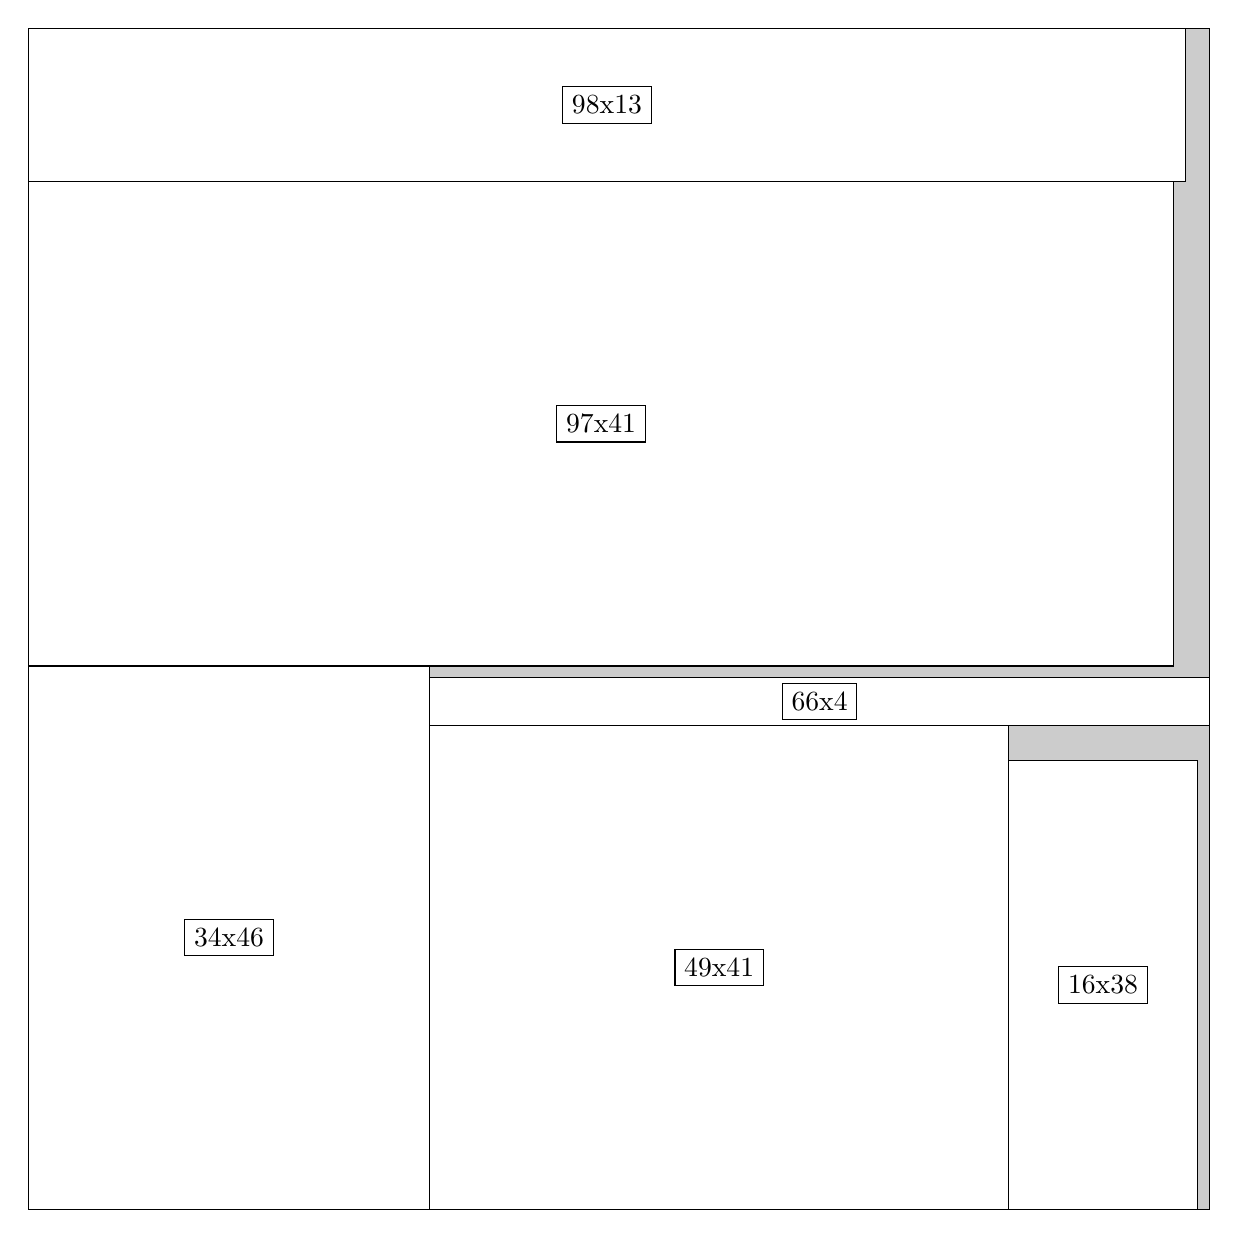
\begin{tikzpicture}[shorten >=1pt,scale=1.0,every node/.style={scale=1.0},->]
\tikzstyle{vertex}=[circle,fill=black!25,minimum size=14pt,inner sep=0pt]
\filldraw[fill=gray!40!white, draw=black] (0,0) rectangle (15.0,15.0);
\foreach \name/\x/\y/\w/\h in {34x46/0.0/0.0/5.1/6.8999999999999995,97x41/0.0/6.8999999999999995/14.549999999999999/6.1499999999999995,49x41/5.1/0.0/7.35/6.1499999999999995,98x13/0.0/13.049999999999999/14.7/1.95,16x38/12.45/0.0/2.4/5.7,66x4/5.1/6.1499999999999995/9.9/0.6}
\filldraw[fill=white!40!white, draw=black] (\x,\y) rectangle node[draw] (\name) {\name} ++(\w,\h);
\end{tikzpicture}


w =34 , h =46 , x =0 , y =0 , v =1564
\par
w =97 , h =41 , x =0 , y =46 , v =3977
\par
w =49 , h =41 , x =34 , y =0 , v =2009
\par
w =98 , h =13 , x =0 , y =87 , v =1274
\par
w =16 , h =38 , x =83 , y =0 , v =608
\par
w =66 , h =4 , x =34 , y =41 , v =264
\par
\newpage


\end{document}